	
\section{Экономико-географическое положение и административно-территориальная структура региона}

\subsection{Географическая зона и природно-климатические условия}

Республика расположена на рубеже Европы и Азии. По природным условиям Башкирию можно разделить на западную, горную и Башкирское Зауралье. Западная Башкирия расположена в пределах Русской равнины. Это наиболее благоприятная для жизни и хозяйственной деятельности человека часть Республики. Горная Башкирия охватывает Южный Урал. Башкирское Зауралье протянулось узкой полосой вдоль восточной границы республики к востоку от Уральских гор. На востоке эта часть Республики сливается с Западно-Сибирской низменностью.

Протяженность территории с севера на юг - 540 км, с запада на восток - 420 км.

Граничит: на юге и юго-западе - с Оренбургской областью, на западе - с Республикой Татарстан, на северо-западе - с Удмуртской Республикой, на севере - с Пермской и Свердловской областями, на востоке - с Челябинской областью.

Климат Башкирии - континентальный с умеренно теплым, иногда жарким летом и холодной зимой. Вытянутые с севера на юг хребты Урала создают резкое различие в климатических условиях на западных и восточных склонах. Средняя температура воздуха составляет плюс $3^{\circ}$С. Самый холодный месяц - январь - характеризуется отрицательными температурами в пределах минус $14,3-16,9^{\circ}$C, самый теплый - июль, когда положительные температуры колеблются от 16,5 до $20,5^{\circ}$С. Безморозный период - 88-90 дней. Наибольшее количество осадков: по западным склонам Урала - 698 мм, в северной части - 550-600 мм, на юге и юго-западе - несколько меньше. Вегетационный период составляет 120-135 дней.

Территория Башкортостана покрыта разветвленной сетью поверхностных водоемов: 1120 рек общей протяженностью более 20 тыс. км и 2720 озер. Большинство из них принадлежат бассейну Каспийского моря. Это реки Урал и Белая. Крупными притоками ее являются реки Уфа, Дема, Сим, Ашкадар, Быстрый Танып. Из других крупных рек - Юрюзань, Ик, Сак-мар, Таналык. Уй и Миасс принадлежат бассейну Северного Ледовитого океана.

Около 5 миллионов гектаров территории республики покрыто лесом. На территории республики находится Башкирский заповедник - расположен в центральной части Южного Урала в излучине реки Белой. Площадь - 72 тысячи гектаров. Создан в 1930 году. Фауна: лось, косуля, медведь, рысь, куница, тетерев, таймень, форель, хариус. В пределах заповедника находится Капова пещера.

\subsection{Природные и экономические ресурсы}

Территория входит в хорошо освоенную и заселенную зону Евразии. По территории проходят важнейшие железнодорожные, автомобильные и трубопроводные магистрали, связывающие европейскую часть РФ с Уралом и Сибирью. С завершением строительства железной дороги Мурапталово — Оренбург Башкортостан получил возможность прямого выхода к Западному Казахстану, Северному Кавказу, низовьям рек Волги, Туркменистану и Узбекистану.

Река Агидель (Белая) — составная часть единой транспортной, глубоководной системы Европейской части России, обеспечивающей доступ РБ к портам Черноморско-Азовского и Балтийского бассейнов. Республика Башкортостан является составной частью Уральского экономического района, уступающего по масштабам индустриального развития лишь Центральному району РФ, находится в соседстве с высокоразвитыми регионами Поволжья и Западно-Сибирского экономического района, недостаточно освоенного, но богатого топливно-энергетическими и минерально-сырьевыми ресурсами.

Разнообразны природные полезные ископаемые Башкирии. Республика богата минеральным сырьем, особенно нефтью, попутным и природным газом в Предуралье (Волго-Уральская нефтегазоносная провинция). Значительны залежи известняков, каменной соли. На востоке республики эксплуатируются месторождения железных и медноколчедановых руд. На юге  бурые угли. Меднорудные месторождения - комплексные и содержат медь, цинк, серу, золото, серебро, кобальт и другие, редкие и рассеянные элементы (основные месторождения: Сибайское, Учалинское).

\subsection{Административно-территориальная структура региона}

Современное административно-территориальное устройство Башкортостана регулируется Законом «Об административно-территориальном устройстве Республики Башкортостан» от 20 апреля 2005 года № 178-з. Во исполнение статьи 16 данного закона утверждён Реестр административно-территориальных единиц и населённых пунктов Республики Башкортостан.

Законом № 178-з (статья 5) установлено, что:

\begin{enumerate}
	\item Статус и наименования административно-территориальных единиц, непосредственно входящих в состав территории Республики Башкортостан, устанавливаются Конституцией Республики Башкортостан.
	\item Территория районов непосредственно подразделяется на территории сельсоветов, поссоветов и городов районного значения.
	\item Города республиканского значения могут иметь в составе своей территории районы в городе (городские районы).
\end{enumerate}

\begin{figure}[h!]
	\begin{center}
		{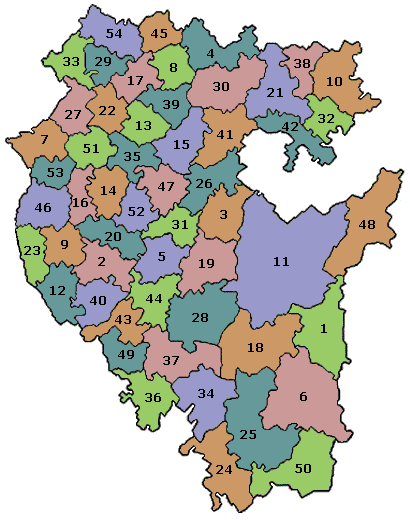
\includegraphics[width=80mm]{pics/alina/admin.png}}
		\caption{Районы Башкоростана}
	\end{center}
\end{figure}


Согласно Закону об административно-территориальном устройстве и утверждённому на его основании реестру административно-территориальных единиц и населённых пунктов, Республика Башкортостан включает следующие административно-территориальные единицы:

\begin{itemize}
	\item районы — 54 — Абзелиловский, Альшеевский, Архангельский, Аскинский, Аургазинский, Баймакский, Бакалинский, Балтачевский, Белебеевский, Белокатайский, Белорецкий, Бижбулякский, Бирский, Благоварский, Благовещенский, Буздякский, Бураевский, Бурзянский, Гафурийский, Давлекановский, Дуванский, Дюртюлинский, Ермекеевский, Зианчуринский, Зилаирский, Иглинский, Илишевский, Ишимбайский, Калтасинский, Караидельский, Кармаскалинский, Кигинский, Краснокамский, Кугарчинский, Кушнаренковский, Куюргазинский, Мелеузовский, Мечетлинский, Мишкинский, Миякинский, Нуримановский, Салаватский, Стерлибашевский, Стерлитамакский, Татышлинский, Туймазинский, Уфимский, Учалинский, Фёдоровский, Хайбуллинский, Чекмагушевский, Чишминский, Шаранский, Янаульский;
	\item города — 21 — Агидель, Баймак, Белебей, Белорецк, Бирск, Благовещенск, Давлеканово, Дюртюли, Ишимбай, Кумертау, Межгорье, Мелеуз, Нефтекамск, Октябрьский, Салават, Сибай, Стерлитамак, Туймазы, Уфа, Учалы, Янаул;
	\item внутригородские районы г. Уфы — 7,
	\item рабочие посёлки (посёлки городского типа) — 2 — Приютово и Чишмы,
	\item сельсоветы — 828
	\item сельские населенные пункты — 4538
\end{itemize}

Существует официальный справочник «Административно-территориальное устройство Республики Башкортостан». В справочнике отражена текущая ситуация об административно-территориальном устройстве, в том числе об административных границах по состоянию на 1 января 2017 года.

Справочник является официальным изданием, в котором содержатся общие сведения о республике, статус и официальные наименования населенных пунктов на башкирском и русском языках, железнодорожных станций и расстояния до них, сведения о расстояниях между населенными пунктами, численности населения.

Издание содержит картографический материал, наглядно отражающий административно-территориальное устройство республики. На карте отражены автодороги, железнодорожные пути, гидрография, крупные водные объекты.

Электронный вариант опубликован на сайте «Республика Башкортостан» в разделе «Справочники» и предназначен для органов государственной власти и местного самоуправления, руководителей организаций и всех тех, кто интересуется административно-территориальным устройством региона.

\begin{figure}[h!]
	\begin{center}
		{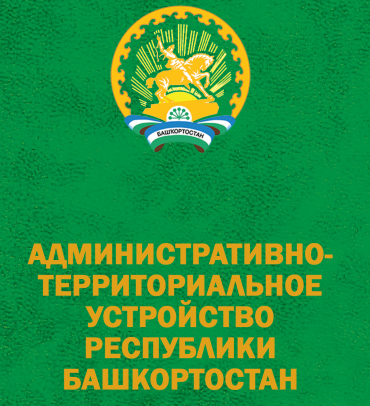
\includegraphics[width=80mm]{pics/alina/spravka.png}}
		\caption{Официальный справочник «Административно-территориальное устройство Республики Башкортостан»}
	\end{center}
\end{figure}

\newpage

\subsection{SWOT-анализ}

\textbf{S}

\begin{itemize}
	\item Территорию республики пересекают железные и автомобильные дороги широтного и меридианального направления, трубопроводы (нефте- и газопроводы)
	\item Река Белая со своим судоходным притоком – рекой Уфой составляет часть Волжско-Камского водного пути, обеспечивает выход в Каспийское, Балтийское, Азовское и Черное моря
\end{itemize}

\textbf{W}

\begin{itemize}
	\item Удаленность от морей и океанов
\end{itemize}

\textbf{O}

\textbf{T}